\documentclass[nohyper,notoc,justified]{tufte-book} 

\usepackage[utf8]{inputenc}
\usepackage[icelandic]{babel}
\usepackage[T1]{fontenc}
\usepackage{amsfonts, amssymb, amsthm, amsmath}
\usepackage{microtype}

\usepackage{tikz}
\usepackage{booktabs}
\usepackage{float}
\usepackage{minted}
\usepackage{listings}
\usepackage{color}

\usepackage{hyperref}

\hypersetup{colorlinks=true,pdfauthor={Eirikur Ernir Thorsteinsson},pdftitle={SQL},linkcolor=blue,urlcolor=blue}

\hyphenpenalty=1000
\hyphenation{Tungu-mál gagna-grunnur gagna-grunna SQL-gagna-grunna gagnagrunns-kerfi}

\newfloat{sql}{bt}{lop}
\floatname{sql}{SQL sýnidæmi}


\makeatletter
% Paragraph indentation and separation for normal text
\renewcommand{\@tufte@reset@par}{%
  \setlength{\RaggedRightParindent}{0pt}%
  \setlength{\JustifyingParindent}{0pt}%
  \setlength{\parindent}{0pt}%
  \setlength{\parskip}{0.4\baselineskip}%
}
\@tufte@reset@par

% Paragraph indentation and separation for marginal text
\renewcommand{\@tufte@margin@par}{%
  \setlength{\RaggedRightParindent}{0pt}%
  \setlength{\JustifyingParindent}{0pt}%
  \setlength{\parindent}{0pt}%
  \setlength{\parskip}{0.3\baselineskip}%
}
\makeatother


\author{Eiríkur Ernir Þorsteinsson}
\title{Notkun gagnasafna - námsefni}
\publisher{Tækniskólinn}
\date{}

\begin{document}

\setcounter{tocdepth}{2}
\setcounter{secnumdepth}{0}

\maketitle

\tableofcontents

\newpage

\chapter{Inngangur}
Skjal þetta er ætlað nemendum til gagns og stuðnings í fyrsta áfanga Tækniskólans er varðar notkun gagnagrunna með SQL.
\section{Hvað er gagnagrunnur?}
Gagnagrunnur\footnote{e. \emph{database}} er, í sinni víðustu skilgreiningu, skipulagt samansafn af upplýsingum.

Í þessari bók munum við skoða svokallaða SQL-gagnagrunna.
Líta má á sem svo að slíkir gagnagrunnar samanstandi fyrst og fremst af \emph{töflum} sem geyma upplýsingarnar. Það að smíða slíkar töflur, breyta þeim og birta úr þeim upplýsingar með SQL er aðalviðfangsefni áfangans.
\section{Hvað er SQL?}
Skammstöfunin SQL stendur fyrir \textbf{S}tructured \textbf{Q}uery \textbf{L}anguage. Skoðum þá skammstöfun nánar.

\emph{Query Language} hefur verið þýtt á íslensku sem \emph{fyrirspurnamál}. SQL er sem sagt mál, líkt og tungumál og forritunarmál, sem nota má til að eiga ákveðin samskipti. SQL er notað til að senda \emph{fyrirspurnir} á gagnagrunnskerfi, oftast í þeim tilgangi að fá upplýsingar frá kerfinu.

\emph{Structured} bendir til þess að málið hafi ákveðna uppbyggingu. Tungumál sem fólk notar til samskipta sín á milli eru oftast mjög sveigjanleg og fær um að koma upplýsingum til skila á marga mismunandi vegu. Tölvur eru hins vegar ekki svo klárar að þær skilji hugtök jafn vel og fólk. Þess vegna þurfa þær fyrirspurnir sem við skrifum að vera á mjög fastmótuðu sniði svo að þær komist til skila. Það að læra SQL snýst að miklu leyti um að læra þetta snið - hvað er leyfilegt innan þess og hvað ekki.
\section{Af hverju SQL?}
Vinnsla gagna er stór hluti af nær öllum stórum tölvukerfum, allt frá einföldum vefsíðum upp í stór bankakerfi. Áratuga reynsla hefur sýnt að SQL er mjög hentugt til slíkrar vinnslu. Oftast er ekki verið að vinna með gagnagrunna til þess eins að eiga gagnagrunna, heldur vegna aflsins sem gagnagrunnar hafa upp á að bjóða sem hluti af stærra kerfi.

Í kafla \ref{undirkafli:php} munum við sjá dæmi um hvernig nota má SQL við heimasíðugerð.
\section{Hvað er gagnagrunnskerfi?}
\label{undirkafli:gagnagrunnskerfi}
Gagnagrunnskerfi\footnote{e. \emph{database management system}} er sá hugbúnaður sem tölva notar til að hafa umsjón með gagnagrunnum. Dæmi í þessari bók miðast við að gagnagrunnskerfið MySQL sé notað.

Yfirlit yfir nokkur gagnagrunnskerfi sem mikið eru notuð má finna í kafla \ref{kafli:itarefni}.
\subsection{Hvernig vinnum við með gagnagrunnskerfi?}
MySQL gagnagrunnskerfi skiptast í \emph{client} og \emph{server}\footnote{orðin client og server hafa verið þýdd sem ``biðlari'' og ``miðlari'' á Íslensku, en þau orð eru í takmarkaðri notkun}. Server sér um úrvinnslu og meðhöndlun gagna. Client tengist servernum og veitir notandanum aðgang að gagnagrunninum.

Til að keyra MySQL-server þarf að setja upp töluverða umgerð á viðkomandi tölvu. Dæmi um hugbúnaðarpakka sem heldur utan um MySQL-server er \href{http://www.apachefriends.org/en/xampp.html}{XAMPP}\footnote{\url{http://www.apachefriends.org/en/xampp.html}}. Ekki verður farið sérstaklega yfir uppsetningu slíkrar umgjörðar hér, en hún er til staðar á vefþjóni\footnote{\url{http://tsuts.tskoli.is/}} tölvudeildar Upplýsingatækniskólans.

Hugbúnaðurinn sem notaður er í Tækniskólanum til að tengjast SQL-servernum er \href{http://www.mysql.com/products/workbench/}{MySQL Workbench}\footnote{\url{http://www.mysql.com/products/workbench/}}. Sá hugbúnaður er þegar upp settur á sýndarvélum nemenda Upplýsingatækniskólans.
\section{Yfirlit}
Í þessum kafla fórum við yfir eftirfarandi atriði:
\begin{itemize}
 \item SQL-gagnagrunnur er samansafn af upplýsingum, skipulagt með töflum.
 \item SQL er fyrirspurnamál, notað til að eiga samskipti við gagnagrunnskerfi.
 \item Forrit geta tengst SQL-gagnagrunnum og notað þá til að sjá um gagnavinnslu. Þetta er gert í stórum stíl í tölvukerfum í dag.
 \item Gagnagrunnskerfi er hugbúnaður sem tölva notar til að hafa umsjón með gagnagrunnum. MySQL er dæmi um gagnagrunnskerfi.
 \item Í þessum áfanga verður gagnagrunnskerfið MySQL notað. Forritið MySQL Workbench verður notað til að tengjast MySQL-server tölvudeildarinnar.
\end{itemize}

\chapter{Fyrstu skrefin í SQL}
\label{kafli:fyrstuskrefin}
SQL er nokkuð sveigjanlegt og yfirgripsmikið mál. 
Margt er að læra, í þessum áfanga er einungis farið yfir lítið brot af því sem viðfangsefnið hefur upp á að bjóða.

Byrjum á að skoða grundvallaraðgerðirnar í SQL - það að búa til töflur, setja í þær gögn og að skoða gögnin aftur.
\section{Töflur}
Gögn í SQL-gagnagrunni má líta á sem raðir í töflum. Því hlýtur mikilvægt skref í því að læra að nota SQL að vera það að skilja uppbyggingu taflna mjög nákvæmlega.

Lítum fyrst á dæmigerða töflu.

\begin{table}
\centering
\caption{Nokkrir starfsmenn Tækniskólans}
\label{tafla:starfsmenn_ts}
\begin{tabular}{lll}
\toprule
Nafn&Starfsheiti&Netfang\\
\midrule
Bjargey G. Gísladóttir&Skólastjóri&bbg@tskoli.is\\
Eiríkur Ernir Þorsteinsson&Kennari&eet@tskoli.is\\
Emil Gautur Emilsson&Kennari&ege@tskoli.is\\
% Donatas Butkus&Tölvuþjónusta&db@tskoli.is\\
Geir Sigurðsson&Kennari&ges@tskoli.is\\
Gunnar Þórunnarson&Kennari&gus@tskoli.is\\
Guðmundur Jón Guðjónsson&Kennari&gjg@tskoli.is\\
Guðrún Randalín Lárusdóttir&Kennari&grl@tskoli.is\\
Hallur Ó. Karlsson&Kennari&hal@tskoli.is\\
Konráð Guðmundsson&Kennari&kng@tskoli.is\\
% Matthias Skúlason&Tölvuþjónusta&matti@tskoli.is\\
Sigurður R. Ragnarsson&Kennari&srr@tskoli.is\\
Snorri Emilsson&Kennari&sem@tskoli.is\\
% Tryggvi Jóhannsson&Kerfisstjóri&tj@tskoli.is\\
Þórarinn J. Kristjánsson&Kennari&tjk@tskoli.is\\
\bottomrule
\end{tabular}
\end{table}
Eins og allar alvöru töflur inniheldur þessi starfsmannatafla annarsvegar \emph{dálkheiti} og hins vegar \emph{gögn}. Dálkheitin eru ``Nafn'', ``Starfsheiti'' og ``Netfang''. Dæmi um upplýsingar eru að til sé starfsmaður sem heitir ``Eiríkur Ernir Þorsteinsson'', sem er ``Kennari'' og hefur netfangið ``eet@tskoli.is''. 

Mikilvægt er að átta sig á þessum mun - hver einasta tafla sem unnið er með inniheldur dálkheiti og gögn, sem eru aðskilin fyrirbrigði. Þetta á augljóslega við ``hefðbundnar'' töflur sem við sjáum á prenti og í forritum á borð við Microsoft Excel. En taktu eftir því að þetta á en líka við töflur sem við skilgreinum með SQL-skipunum.

Þegar töflur eru sýndar á prenti er venjan að dálkheitin komi fram í fyrstu línu töflunnar (og oftast aðskilin gögnunum með striki). Gögnin koma fram í næstu línum.

Þegar SQL er notað til að lýsa töflum eru dálkheitin og aðrar upplýsingar sem skilgreina töfluna sjálfa búnar til með sérstökum skipunum. Aðrar skipanir eru notaðar til að vinna með gögnin sjálf. Við sjáum dæmi um þessar skipanir í undirkaflanum \nameref{undirkafli:synidaemi_i_sql}. 6\footnote{Betur verður farið í muninn á þessum skipunum í kafla \ref{kafli:uppfaera}}
\section{Fyrirspurnir}
Ekki er mikið gagn í því að geyma upplýsingar í töfluformi nema að hægt sé að ná í þær aftur.

Einfalt er að fletta upp upplýsingum í litlum töflum á borð við töflu \ref{tafla:starfsmenn_ts}. Viljum við t.d. komast að því hver er með netfangið ``kng@tskoli.is'' dugar okkur að láta augun reika yfir töfluna þar til við rekumst á netfangið og líta svo í starfsmannadálkinn.

Væri taflan örlítið stærri væri verkefnið strax erfiðara. Væri taflan á stærð við símaskrána væri það nær ómögulegt.

Slíkar uppflettingar, stórar og smáar, eru sérsvið SQL. Þær eru nefndar \emph{fyrirspurnir} og eru framkvæmdar með mjög mikilvægri SQL-skipun sem heitir \emph{SELECT}. Við sjáum dæmi um SELECT-skipanir í undirkaflanum \nameref{undirkafli:synidaemi_i_sql} og kynnumst þeim náið í kafla \ref{kafli:select}.
\section{Gagnagrunnar}
Ef upplýsingar eru geymdar í töflum, hvað er þá gagnagrunnur?

Gagnagrunnur heldur utan um töflur, eina eða fleiri. Hann bindur þær saman í eina heild og myndar um þær umgjörð.
\begin{marginfigure}
\centering
\caption{Uppbygging gagnagrunns}
\label{mynd:uppbygging}
\color{red} Hingað kemur falleg mynd af uppbyggingu gagnagrunna.
\end{marginfigure}

\section{Sýnidæmi í SQL}
\label{undirkafli:synidaemi_i_sql}
Skoðum hvernig búa má til töflu \ref{tafla:starfsmenn_ts} með SQL, setja í hana gögn og sækja gögnin aftur. 

Eins og fram hefur komið þarf til þess að nota SQL-skipanir.

\begin{example}[h]
\caption{CREATE skipun fyrir starfsmannatöfluna}
\label{sql:k2d1}
\centering
\sql{sql/k2d1.sql}
\end{example}

Skipunina til að skilgreina töfluna má sjá á SQL-sýnidæmi \ref{sql:k2d1}. Þetta er mjög dæmigerð skipun til að búa til töflu. Þar kemur fram hvað gera skal (búa til töflu $\rightarrow$ \verb|CREATE TABLE|) og hver dálkheitin eru (nafn, Starfsheiti og netfang). Í kafla \ref{kafli:uppsetningtaflna} skoðum við hin orðin sem koma fyrir í skipuninni og í kafla \ref{undirkafli:keyrslaiworkbench} sjáum við hvernig koma má skipuninni í gagnið.

Hér ber að athuga að enn eru engin gögn komin inn í töfluna. Það má gera með skipuninni í SQL-sýnidæmi \ref{sql:k1d2}.

\begin{example}[h]
\caption{INSERT skipun fyrir starfsmannatöfluna}
\label{sql:k2d2}
\centering
{\small
\sql{sql/k2d2.sql}
}
\end{example}

Til að sækja gögn úr töflunni þarf síðan að framkvæma fyrirspurn. Dæmi um fyrirspurn (SQL-skipun) sem finnur nafn þess starfsmanns sem er með netfangið ``kng@tskoli.is'' má sjá á sýnidæmi \ref{sql:k2d3}.

\begin{example}[h]
\caption{SELECT skipun sem finnur Konráð kennara í starfsmannatöflunni}
\label{sql:k2d3}
\centering
\sql{sql/k2d3.sql}
\end{example}

\section{Keyrsla í MySQL Workbench}
\label{undirkafli:keyrslaiworkbench}
Lítum örstutt á hvernig nota má MySQL Workbench til að búa til okkar fyrstu töflu með SQL.

Um nokkur skref er að ræða.
\begin{enumerate}
 \item Ræsa þarf forritið. Við það birtist upphafsskjár, líkur þeim sem sjá má á mynd \ref{mynd:workbench-upphafsskjar}.\footnote{Útlit MySQL Workbench er eðli málsins samkvæmt örlítið mismunandi eftir stýrikerfum og útgáfum á forritinu. Skjáskotin eru tekin af Workbench útgáfu 6.0, á Linux vél.}
 \item Mynda þarf tengingu við MySQL-server. Henni þarf að gefa nafn, IP-tölu MySQL serversins, notandanafn og lykilorð.\footnote{Nemendur Tölvudeildar Tækniskólans skulu biðja kennarann um þessar upplýsingar.} Sjá mynd \ref{mynd:workbench-login}.
 \item Búa þarf til nýjan gagnagrunn á MySQL-servernum á skjánum sem birtist eftir að tengingin er mynduð. Það er einfaldast að gera með svokallaðri \verb|CREATE DATABASE| skipun, slegin inn í aðalgluggann - sjá mynd \ref{mynd:workbench-create-db}. Þegar þessu er lokið höfum við keyrt okkar fyrstu SQL-skipun!
 \item Skipunin í sýnidæmi \ref{sql:k2d1} er slegin inn í aðalgluggann og keyrð. Taflan er þá komin inn!
\end{enumerate}
Ávallt má gera ráð fyrir að SQL-sýnidæmi í þessari bók megi keyra með hliðstæðum hætti - í aðalglugga MySQL Workbench. T.d. mætti keyra sýnidæmi \ref{sql:k1d2} og \ref{sql:k2d3} á þann hátt.

\begin{figure*}
\caption[Upphafsskjár MySQL Workbench]{Upphafsskjár MySQL Workbench. Örin vísar á hnapp sem nota má til að búa til nýja tengingu.}
\label{mynd:workbench-upphafsskjar}
\centering
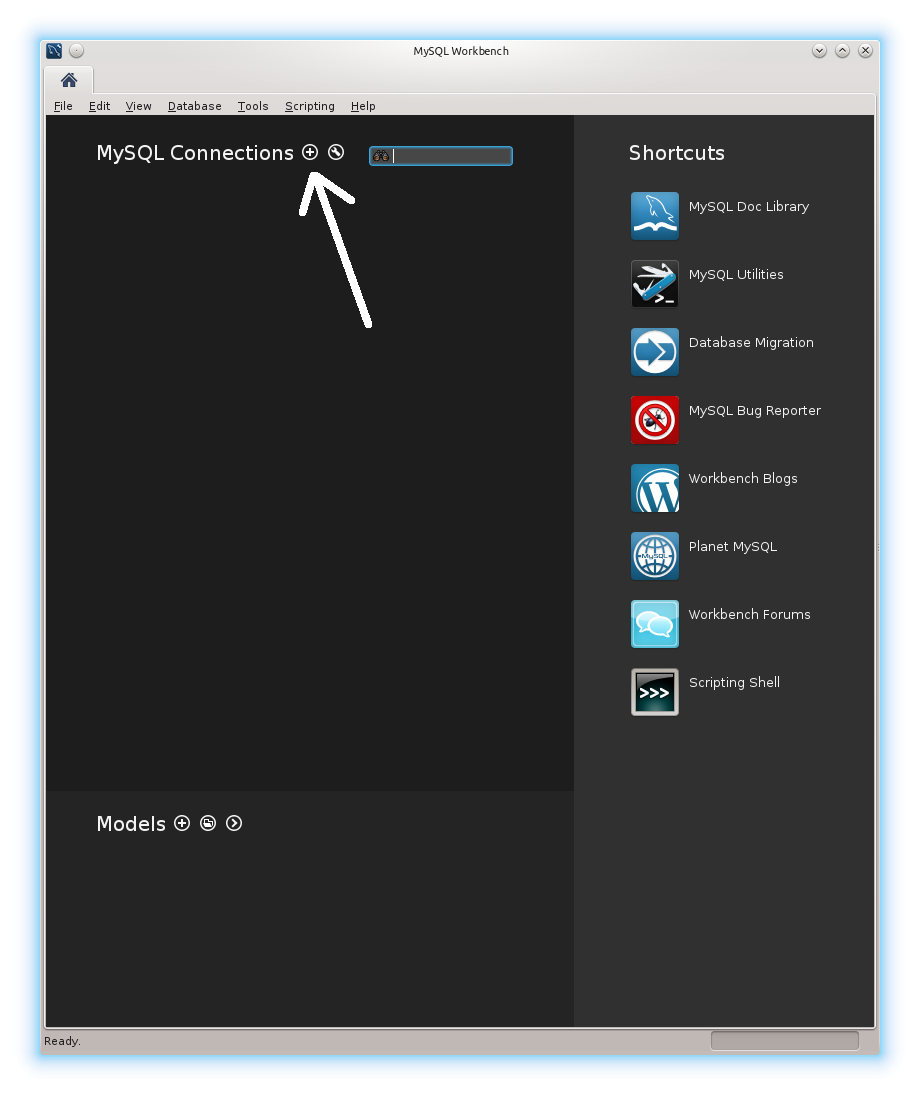
\includegraphics[width=\linewidth]{myndir/workbench-upphafsskjar-or}
\end{figure*}

\begin{figure*}
\caption[Tengingarskjár MySQL Workbench]{Tengingarskjár MySQL Workbench. Hér er verið að búa til tenginguna ``Prufutenging'', sem tengist MySQL-þjóni sem keyrir á sömu tölvu og Workbench-inn (127.0.0.1) með notandanafninu ``root''.}
\label{mynd:workbench-login}
\centering
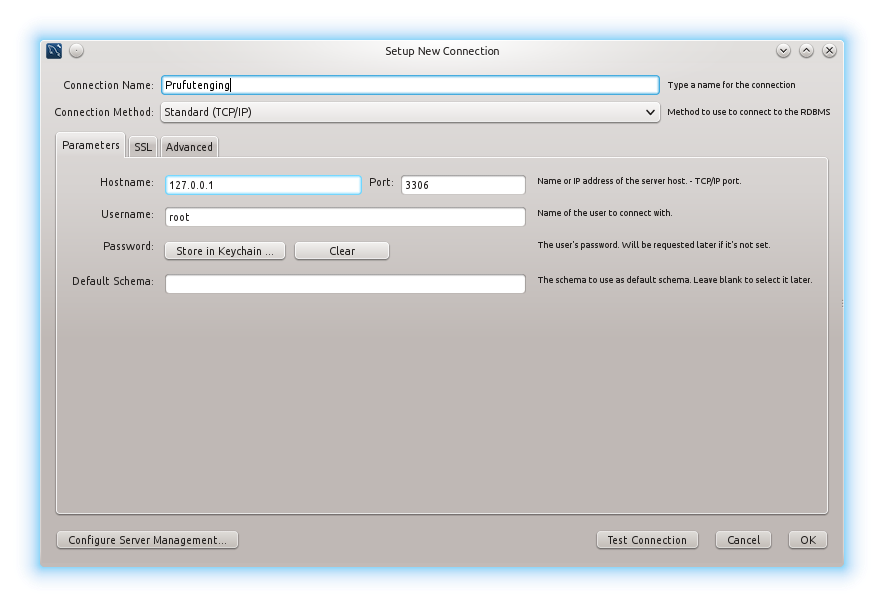
\includegraphics[width=\linewidth]{myndir/workbench-login}
\end{figure*}

\begin{figure*}
\caption[Nýr gagnagrunnur]{Nýr gagnagrunnur búinn til með MySQL Workbench. Efri örin vísar á hnappinn sem ýta þarf á til að keyra SQL-skipunina. Neðri örin vísar á lista af gagnagrunnum sem sýnilegir eru á servernum. Birtist gagnagrunnurinn sem búinn er til ekki um leið og skipunin er keyrð, hægri-smellið þá á listann og ``refresh''ið hann.}
\label{mynd:workbench-create-db}
\centering
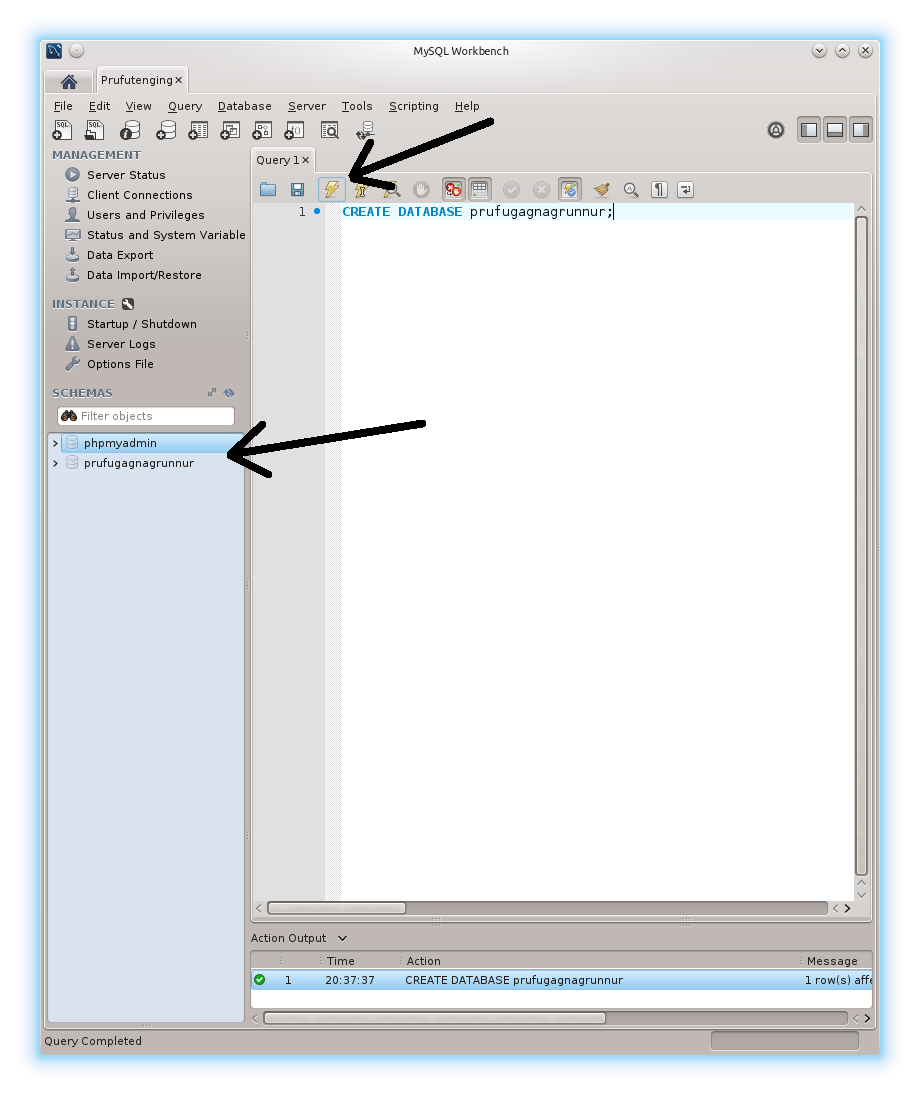
\includegraphics[width=0.8\linewidth]{myndir/workbench-create-db-or}
\end{figure*}

\begin{figure*}
\caption[Ný tafla]{Ný tafla búin til með MySQL Workbench. Skipunin er slegin inn í aðalgluggann og keyrð með ``eldingarhnappnum'' eins og skipunin á mynd \ref{mynd:workbench-create-db}.}
\label{mynd:workbench-create-table}
\centering
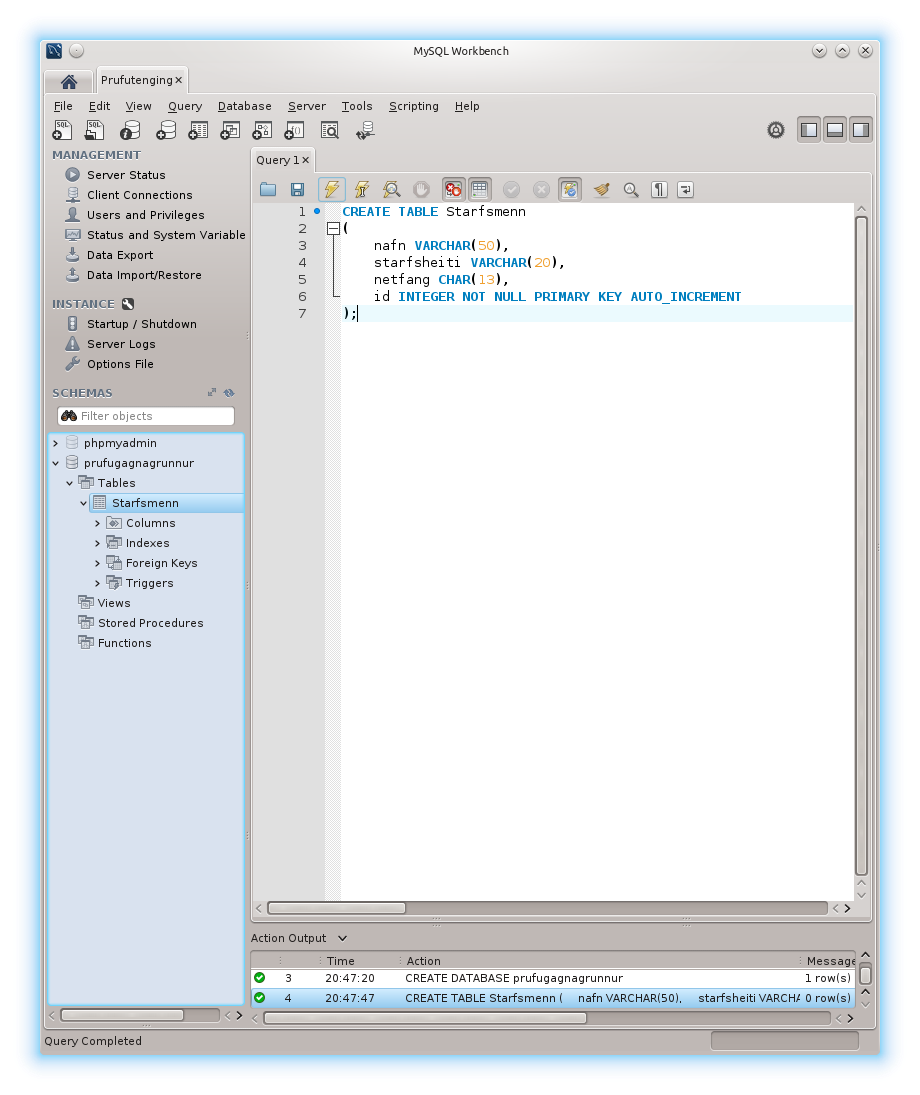
\includegraphics[width=0.8\linewidth]{myndir/workbench-create-table}
\end{figure*}

\section{Yfirlit}
Í þessum kafla fengum við örstutta kynningu því hvernig SQL-gagnagrunnar eru uppbyggðir og hvernig við getum átt við þá samskipti. 

Helstu atriðin eru:
\begin{itemize}
 \item Gögn í SQL-gagnagrunni má líta á sem raðir í töflum.
 \item SQL-skipanir eru notaðir til að skilgreina töflur og setja í þær gögn.
 \item Fyrirspurnir eru notaðar til að sækja gögn úr gagnagrunnum. Fyrirspurnir eru sérstök gerð SQL-skipana.
 \item SQL-skipanir má keyra úr aðalglugga MySQL Workbench.
\end{itemize}
Athuga ber að við höfum ekki farið yfir uppbyggingu skipananna. Það að læra á skipanirnar sjálfar er viðfangsefni næstu kafla.

\chapter{Uppsetning á töflum}
\section{Að búa til töflu} % CREATE
\section{Helstu gagnagerðir} % INT, VARCHAR, CHAR, DATE
\section{Tóm gildi} % NULL, NOT NULL
\section{Innsetning gagna} % INSERT
\section{Að eyða töflum} % DROP

\chapter{Fyrirspurnir}
\label{kafli:select}
\section{SELECT, FROM og WHERE}
\section{LIKE og ``wildcards''}
\section{AND, OR og IN}
\section{Helstu einindaföll}
\subsection{LENGTH}
\subsection{ROUND}
\subsection{UCASE og LCASE}
\section{Helstu samsteypuföll}
\subsection{SUM og AVG}
\subsection{MIN og MAX}
\subsection{COUNT}
\section{GROUP BY}
\section{ORDER BY}

\chapter{Að setja upp gagnagrunn}
\section{Aðallyklar} % PRIMARY KEY
\section{Margar töflur í sama gagnagrunninum}
\section{Aðkomulyklar} % FOREIGN KEY
\section{Tengingar} % 1-1, 1-N, N-N

\chapter{Gagnavinnsla með mörgum töflum}
\section{INNER JOIN}
\section{OUTER JOIN}
\section{Undirfyrirspurnir}

\chapter{Að uppfæra gagnagrunna}
\label{kafli:uppfaera}
\section{DDL og DML}
\section{Að breyta töflum}
\section{Að breyta gögnum}
\section{Að eyða gögnum}

\chapter{Ítarefni}
\label{kafli:itarefni}
\section{Views}
\section{Yfirlit yfir helstu gagnagrunnskerfi}
\subsection{MySQL}
\subsection{SQLite}
\subsection{PostgreSQL}
\subsection{Microsoft SQL Server}
\subsection{Oracle Database}
\section{Venslalíkanið}
\section{Að tengjast gagnagrunni með PHP}
\end{document}